%=============================
\chapter{La structure d'arbre}
%=============================

{\itshape La structure d'arbre trouve de nombreuses utilités en informatique~: 
évaluation d'expressions algébriques, modélisation de l'inclusion d'ensembles,
d'organisations hiérarchiques, de schémas en analyse, d'arbre généalogique, 
arborescence des dossiers dans un système d'exploitation, variables 
structurées C et en Cobol...}
\begin{center}
	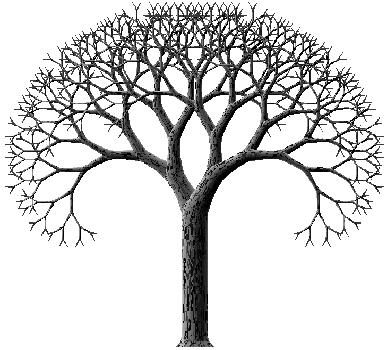
\includegraphics[width=4.494cm,height=4.045cm]{image/a2012Logique2eme-img028.png}
\end{center}
	

%===================================
\section{Définition et terminologie}
%===================================

	\subsection{arbre}
	%=================
		En informatique, un \textbf{arbre} est une structure de données 
		constituée de \textbf{n{\oe}uds} assemblés par \textbf{niveaux}. 
		C'est un graphe orienté connexe dont chaque arc relie un 
		\textbf{n{\oe}ud père} à un \textbf{n{\oe}ud fils}. 
		Chaque n{\oe}ud peut posséder un nombre quelconque de fils ; 
		un n{\oe}ud sans fils est appelé \textbf{n{\oe}ud terminal} 
		ou \textbf{feuille}.

		Chaque n{\oe}ud possède un et un seul père, sauf la \textbf{racine}, 
		située au sommet de l'arbre, qui ne possède pas de n{\oe}ud père. 
		Les n{\oe}uds autres que la racine ou les feuilles sont appelés 
		\textbf{n{\oe}uds internes}. Deux n{\oe}uds ayant le même père 
		sont des \textbf{frères}.

		\begin{center}
		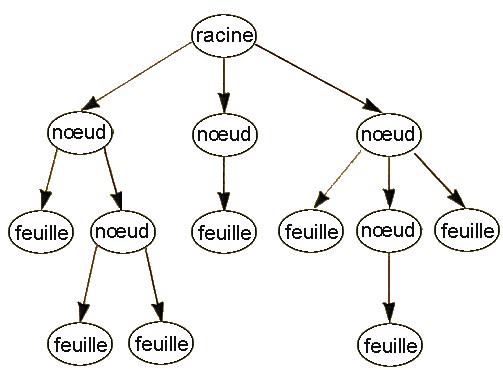
\includegraphics[width=9.036cm,height=6.636cm]{image/a2012Logique2eme-img029.png} 
		\end{center}
		
		\textit{Attention~: ne pas confondre l'arbre au sens informatique 
		et celui étudié dans la théorie des graphes au cours de mathématique ; 
		en théorie des graphes, un arbre est défini comme un graphe sans 
		circuit et est dépourvu de toute structure hiérarchique. L'arbre au sens
		informatique est aussi appelé arbre enraciné.}

		On peut aussi définir l'arbre de manière récursive~: 
		c'est une structure soit vide, soit composée d'un n{\oe}ud auquel
		est rattaché un ensemble fini d'arbres disjoints. 
		Notez que cette définition récursive correspond bien à la réalité de
		ce qu'est un arbre dans la nature !

	\subsection{Niveau et hauteur}
	%=============================

		Le \textbf{niveau} (ou \textbf{profondeur}) d'un n{\oe}ud 
		est la distance qui le sépare de la racine. Il en découle que
		le niveau de la racine est 0, et le niveau de tout autre 
		n{\oe}ud est égal au niveau de son père augmenté de 1.

		\begin{center}
		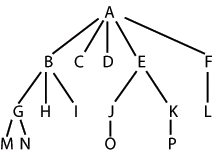
\includegraphics[width=5.092cm,height=3.819cm]{image/a2012Logique2eme-img030.png}
		\end{center}

		{\itshape	
		Exemple~: dans le graphe ci-dessus, les niveaux sont les suivants~: 
		0 pour A, 1 pour B, C, D, E, F, 2 pour G, H, I, J, K, L 
		et 3 pour M, N, O, P.}

		Inversement, la \textbf{hauteur} d'un n{\oe}ud est la distance entre 
		ce n{\oe}ud et sa descendance la plus éloignée~: la hauteur d'une 
		feuille est donc 0 et la hauteur de tout autre n{\oe}ud est le maximum 
		de la hauteur de ses fils augmenté de 1. La \textbf{hauteur d'un arbre} 
		est la hauteur de sa racine, et correspond aussi à son niveau maximum. 
		Elle n'est pas définie pour un arbre vide.

		{\itshape
		Pour le même graphe ci-dessus, les n{\oe}uds C, D, H, I, L, M, N, O et P 
		ont une hauteur 0 (ce sont les feuilles de l'arbre). 
		La hauteur de G, J, K et F est 1, celle de B et E est 2 
		et enfin A est à hauteur 3, qui correspond aussi à la hauteur de l'arbre.}

		Les n{\oe}uds d'un arbre contiennent de l'information, 
		appelée parfois «~étiquette~». L'étiquette peut être un simple
		entier ou une variable structurée plus complexe, l'instance 
		d'un objet, un pointeur, etc. Le type de l'information
		détermine le type de l'arbre~: on parlera d'un arbre 
		d'entiers, de chaines et en général d'arbre de type T.
	
	\subsection{Arbres particuliers}
	%===============================
	
		Un arbre dont tout n{\oe}ud possède au plus un descendant 
		est appelé \textbf{arbre dégénéré}.

		Un arbre dont tout n{\oe}ud possède au plus un nombre 
		déterminé \textit{n} de descendants est appelé \textbf{arbre
		}\textbf{\textit{n}-aire}. 
		
		Si dans un arbre \textit{n}-aire, toutes les feuilles ont 
		le même niveau, et si la racine et tous les n{\oe}uds
		internes ont le même nombre de fils, l'arbre est alors 
		\textbf{complet}. En particulier, un arbre dégénéré est complet ! 
		Le schéma ci-dessus montre un arbre «~2-aire~» complet~: 
		chaque n{\oe}ud non terminal à 2 fils, et toutes les
		feuilles sont au même niveau.

		\begin{center}
		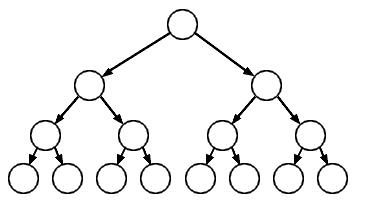
\includegraphics[width=6.918cm,height=3.909cm]{image/a2012Logique2eme-img031.png}
		\end{center}


%============================
\section{Parcours d'un arbre}
%============================

	Il y a plusieurs façons de parcourir un arbre, le choix du parcours 
	dépendant du type de traitement des informations de l'arbre.

	\subsection{Parcours en largeur}
	%===============================

		Le parcours en largeur, aussi nommé \textbf{parcours par niveau}, 
		consiste à visiter les n{\oe}uds dans l'ordre de leur niveau~: 
		la racine, puis les n{\oe}uds de niveau 1, ceux de niveau 2 
		et ainsi de suite. L'ordre de parcours des n{\oe}uds pour 
		un niveau donné est déterminé de manière récursive par 
		l'ordre des n{\oe}uds parents. Sur les schémas, l'ordre 
		des n{\oe}uds correspond à leur disposition de gauche à droite.

		{\itshape
		Exemple~: pour le graphe suivant, l'ordre de visite des n{\oe}uds 
		par le parcours par niveau est A, B, C, D, E, F, G, H,
		I, J, K, L, M, N, O, P.}

		\begin{center}
		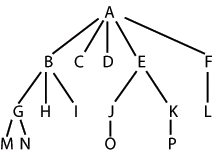
\includegraphics[width=5.821cm,height=4.366cm]{image/a2012Logique2eme-img032.png}
		\end{center}
	
	\subsection{Parcours en profondeur}
	%==================================
	
		Il s'agit d'un parcours récursif sur les n{\oe}uds de l'arbre~: 
		partant de la racine, on visite tous ses fils, mais on
			ne passe à un n{\oe}ud frère qu'après avoir visité tous les 
			fils du n{\oe}ud courant, et ceci récursivement. Il y a
			deux possibilités de traitement des n{\oe}uds~: si le 
			n{\oe}ud courant est traité avant ses fils, on parle de
			\textbf{parcours préfixé}. Si le n{\oe}ud courant est 
			traité après ses fils, on parle de \textbf{parcours postfixé}.

			{\itshape
			Pour le graphe ci-dessus, le parcours en profondeur préfixé donne~: 
			A, B, G, M, N, H, I, C, D, E, J, O, K, P, F, L. 
			Le parcours en profondeur postfixé donne~: 
			M, N, G, H, I, B, C, D, O, J, P, K, E, L, F, A.}
			

%=====================================
\section{Implémentation orienté objet}
%=====================================

	Un arbre est déterminé par sa racine qui est un n{\oe}ud de type T. 
	Chaque n{\oe}ud contient de l'information (attribut
	valeur de type T) et doit permettre de passer à ses 
	descendants (le 1\textsuperscript{er}, le 2\textsuperscript{e},
	etc.) d'où également un attribut de type Liste qui permet 
	d'accéder par position à chacun des fils (Liste d'éléments de
	type N{\oe}ud<T>). L'implémentation de l'arbre est donc 
	déterminée par la donnée des deux classes suivantes~: 
	
	\cadre{
		\begin{pseudo}
			\Class{N{\oe}ud<T>}
				\Private
					\Decl valeur~: T
					\Decl ListeFils~: Liste<{N{\oe}ud<T>}>
				\Public
					\ConstrSign{N{\oe}ud<T>}{val~: T}
					\LComment construit un n{\oe}ud sans fils
					\MethodSign{getValeur}{}{T}
					\MethodSign{setValeur}{val~: T}{}
					\MethodSign{getNbFils}{}{entier}
					\MethodSign{getFils}{i~: entier}{N{\oe}ud<T>}
					\MethodSign{setFils}{i~: entier, fils~: N{\oe}ud<T>}{}
					\MethodSign{ajouterFils}{fils~: N{\oe}ud<T>}{}
					\RComment ajout à la fin de la liste des fils
					\MethodSign{supprimerFils}{i~: entier}{}
			\EndClass
		\end{pseudo}
	}
	
	\cadre{
		\begin{pseudo}
			\Class{Arbre<T>}
				\Private
					\Decl racine : N{\oe}ud<T>
				\Public
					\ConstrSign{Arbre<T>}{}
					\LComment construit un arbre vide
					\MethodSign{getRacine}{}{N{\oe}ud<T>}
					\MethodSign{setRacine}{racine~: N{\oe}ud<T>}{}
			\EndClass
		\end{pseudo}
	}

	Les contenus des méthodes de la classe N{\oe}ud<T> se laissent 
	deviner aisément ; les cinq dernières méthodes consistent à appliquer 
	respectivement sur l'attribut \textbf{ListeFils} 
	les méthodes \textit{taille}, \textit{get}, \textit{set}, 
	\textit{ajouter} et \textit{supprimer} de la classe Liste.

	Noter que -- comme pour la liste chainée monodirectionnelle -- 
	on ne peut voyager dans un arbre que dans un seul sens,
	de la racine vers les feuilles, il n'y a pas de lien 
	d'un n{\oe}ud vers son n{\oe}ud père. Le rajout de ce lien serait
	une possibilité d'implémentation (comme pour la liste bidirectionnelle) 
	mais il n'est pas nécessaire pour la plupart des algorithmes 
	de parcours qui fonctionnent essentiellement de manière récursive 
	(pour les parcours en profondeur) ou à l'aide d'une file 
	(parcours en largeur). Nous donnons à titre d'exemple le détail 
	de ces algorithmes de parcours.

%==========================================
\section{Exemple~: algorithmes de parcours}
%==========================================

	\subsection{Parcours en largeur}
	%===============================
		
		Il n'existe pas de version récursive pour ce parcours. 
		La solution ci-dessous utilise une file où sont placés les fils
		des n{\oe}uds visités successifs.
		
		\cadre{
			\begin{pseudo}
				\Module{parcoursLargeur}{monArbre~: Arbre<T>}{}
					\Decl maFile~: File<{N{\oe}ud<T>}>
					\Decl n{\oe}udCourant~: N{\oe}ud<T>
					\Decl i~: entier
					\Let maFile \Gets \K{nouveau}	File<{N{\oe}ud<T>}>
					\If{monArbre.getRacine( ) ${\neq}$ rien}
						\Stmt maFile.enfiler(monArbre.getRacine( ))
					\EndIf
					\While{NON maFile.estVide( )}
						\Let n{\oe}udCourant \Gets maFile.défiler( )
						\LComment traitement du n{\oe}ud courant
						\For{i \K{de} 1 \K{à} n{\oe}udCourant.getNbFils( )}
							\Stmt maFile.enfiler(n{\oe}udCourant.getFils(i))
						\EndFor
					\EndWhile
				\EndModule
			\end{pseudo}
		}

	\subsection{Parcours en profondeur}
	%==================================

		Ce parcours est essentiellement récursif. Il faut ici un module 
		façade, qui appelle le module récursif avec la racine de
		l'arbre comme première valeur du paramètre. Noter l'emplacement 
		du traitement du n{\oe}ud courant selon le parcours
		préfixé ou postfixé.
		
		\cadre{
			\begin{pseudo}
				\Module{parcoursProfondeur}{monArbre~: Arbre<T>}{}
					\If{monArbre.getRacine( ) ${\neq}$ rien}
						\Stmt parcoursProfondeurRécursif(monArbre.getRacine( ))
					\EndIf
				\EndModule
			\end{pseudo}
		}
		
		\cadre{
			\begin{pseudo}
				\Module{parcoursProfondeurRécursif}{n{\oe}udCourant~: N{\oe}ud<T>}{}
					\Decl i~: entier
					\LComment instructions de traitement du n{\oe}ud courant 
					si parcours préfixé
					\For{i \K{de} 1 \K{à} n{\oe}udCourant.getNbFils( )}
						\Stmt parcoursProfondeurRécursif(n{\oe}udCourant.getFils(i))
					\EndFor
					\LComment instructions de traitement du n{\oe}ud courant 
					si parcours postfixé
				\EndModule
			\end{pseudo}
		}


%======================
\section{Arbre binaire}
%======================

	\subsection{L'arbre binaire}
	%===========================
		
		L'\textbf{arbre binaire} est un type d'arbre particulier~: 
		chaque n{\oe}ud possède au plus deux descendants qui sont
		appelés \textbf{fils gauche} et \textbf{fils droit}. Les 
		deux sous-arbres attachés à un n{\oe}ud donné sont appelés
		sous-arbre gauche et sous-arbre droit.

		\begin{center}
		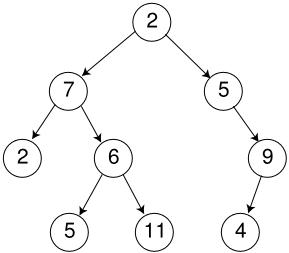
\includegraphics[width=4.671cm,height=4.129cm]{image/a2012Logique2eme-img033.jpg} 
		\end{center}
		
		Attention, l'arbre binaire n'est pas un cas particulier d'arbre 
		\textit{n}-aire (avec la valeur 2 pour \textit{n}), car les deux fils 
		d'un n{\oe}ud sont liés à une orientation~(gauche ou droit). 
		Dans le cas où un n{\oe}ud ne possède qu'un fils, il faut clairement 
		indiquer dans le schéma d'un arbre binaire s'il s'agit du fils 
		gauche ou droite, on ne peut donc jamais représenter un fils 
		à la verticale du père.

		Ainsi, dans l'exemple ci-dessus, le n{\oe}ud 9 est le fils 
		droit du n{\oe}ud 5, et le n{\oe}ud 4 est le fils gauche du
		n{\oe}ud 9.

	\subsection{Implémentation}
	%==========================
		
		Elle se déduit de l'implémentation de l'arbre «~quelconque~». 
		Pour le n{\oe}ud d'arbre binaire, la liste des fils est
		remplacée par deux liens~: un vers le fils gauche et un autre 
		vers le fils droit.

		\cadre{
			\begin{pseudo}
				\Class{N{\oe}udBinaire<T>}
					\Private 
						\Decl valeur~: T
						\Decl gauche~: <{N{\oe}udBinaire<T>}>
						\Decl droit~: <{N{\oe}udBinaire<T>}>
					\Public 
						\ConstrSign{N{\oe}udBinaire<T>}{val~: T}
						\RComment construit un n{\oe}ud sans fils
						\MethodSign{getValeur}{}{T}
						\MethodSign{setValeur}{val~: T}{}
						\MethodSign{getGauche}{}{N{\oe}udBinaire<T>}
						\MethodSign{setGauche}{fils~: N{\oe}udBinaire<T>}{}
						\MethodSign{getDroit}{}{N{\oe}udBinaire<T>}
						\MethodSign{setDroit}{fils~: N{\oe}udBinaire<T>}{}
				\EndClass
			\end{pseudo}
		}
		
		\cadre{
			\begin{pseudo}
				\Class{ArbreBinaire<T>}
					\Private
						\Decl racine~: N{\oe}udBinaire<T>
					\Public 
						\ConstrSign{ArbreBinaire<T>}{}
						\RComment construit un arbre vide
						\MethodSign{getRacine}{}{N{\oe}udBinaire<T>}
						\MethodSign{setRacine}{r~: N{\oe}udBinaire<T>}{}
				\EndClass
			\end{pseudo}
		}


%====================================
\section{Parcours de l'arbre binaire}
%====================================

	\subsection{Parcours en largeur}
	%===============================

		La boucle «~pour~» du parcours de l'arbre «~quelconque~» 
		est remplacée ici par la mise en file de chacun des fils du
		n{\oe}ud courant. Il faut toutefois prendre garde de ne 
		pas mettre de lien vide dans la file.
		
		\cadre{
			\begin{pseudo}
				\Module{parcoursLargeur}{monArbre~: ArbreBinaire<T>}{}
					\Decl maFile~: File<{N{\oe}udBinaire<T>}>
					\Decl n{\oe}udCourant~: N{\oe}udBinaire<T>
					\Decl i~: entier
					\Let maFile \Gets \K{nouveau} File<{N{\oe}udBinaire<T>}>
					\If{monArbre.getRacine( ) ${\neq}$ rien}
						\Stmt maFile.enfiler(monArbre.getRacine( ))
					\EndIf
					\While{NON maFile.estVide( )}
						\Let n{\oe}udCourant \Gets maFile.défiler( )
						\LComment traitement du n{\oe}ud courant
						\If{n{\oe}udCourant.getGauche( ) ${\neq}$ rien}
							\Stmt maFile.enfiler(n{\oe}udCourant.getGauche( ))
						\EndIf
						\If{n{\oe}udCourant.getDroit( ) ${\neq}$ rien}
							\Stmt maFile.enfiler(n{\oe}udCourant.getDroit( ))
						\EndIf
					\EndWhile
				\EndModule
			\end{pseudo}
		}
	
	\subsection{Parcours en profondeur}
	%==================================
	
		Pour les arbres binaires, aux parcours en profondeur préfixé 
		et postfixé s'ajoute le \textbf{parcours infixé}~: le
		traitement d'un n{\oe}ud se fait entre les parcours de son 
		sous-arbre gauche et de son sous-arbre droit.
		
		\cadre{
			\begin{pseudo}
				\Module{parcoursProfondeur}{monArbre~: ArbreBinaire<T>}{}
					\Stmt parcoursProfondeurRécursif(monArbre.getRacine( ))
				\EndModule
			\end{pseudo}
		}
		
		\cadre{
			\begin{pseudo}
				\Module{parcoursProfondeurRécursif}{n{\oe}udCourant~: N{\oe}udBinaire<T>}{}
					\If{n{\oe}udCourant ${\neq}$ rien}
						\LComment instructions de traitement du n{\oe}ud courant si parcours préfixé (ou RGD)
						\Stmt parcoursProfondeurRécursif(n{\oe}udCourant.getGauche( ))
						\LComment instructions de traitement du n{\oe}ud courant si parcours infixé (ou GRD)
						\Stmt parcoursProfondeurRécursif(n{\oe}udCourant.getDroit( ))
						\LComment instructions de traitement du n{\oe}ud courant si parcours postfixé (ou GDR)
					\EndIf
				\EndModule
			\end{pseudo}
		}
		
		{\itshape
		Par exemple, pour l'arbre binaire représenté ci-dessous~:}

		\begin{center}
		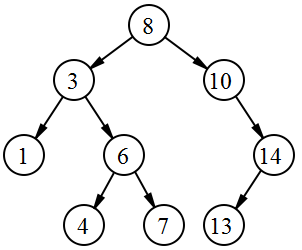
\includegraphics[width=4.457cm,height=3.687cm]{image/a2012Logique2eme-img034.png}
		\end{center}
		
		{\itshape
		les ordres de traitements sont les suivants~:
		
		\begin{itemize}
			\item {
				parcours en largeur~: 8, 3, 10, 1, 6, 14, 4, 7, 13}
			\item {
				parcours en profondeur préfixé~: 8, 3, 1, 6, 4, 7, 10, 14, 13}
			\item {
				parcours en profondeur infixé~: 1, 3, 4, 6, 7, 8, 10, 13, 14}
			\item {
				parcours en profondeur postfixé~: 1, 4, 7, 6, 3, 13, 14, 10, 8}
		\end{itemize}
		}
		
		
%==============================
\section{Arbre binaire ordonné}
%==============================

	\subsection{Définition}
	%======================

	Un arbre binaire est ordonné si pour tout n{\oe}ud, toutes les valeurs 
	de son sous-arbre gauche sont inférieures ou égales à la valeur 
	du n{\oe}ud, et toutes les valeurs de son sous-arbre droit sont 
	strictement supérieures à la valeur du n{\oe}ud.

	{\itshape Exemple~:}

	\begin{center}
	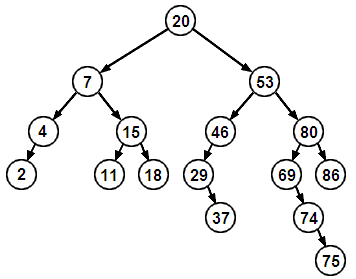
\includegraphics[width=6.994cm,height=5.486cm]{image/a2012Logique2eme-img035.png}
	\end{center}
	
	Cette structure se prête assez bien aux opérations de recherche, 
	d'ajout, de suppression car elle permet de localiser
	rapidement le n{\oe}ud où doit être exécuté l'opération, 
	tout en offrant une souplesse dans ses modifications (comme
	pour une liste chainée). La recherche s'apparente à la 
	recherche dichotomique dans un tableau, et si l'arbre est
	\textit{équilibré} (pour une définition précise de ce terme, 
	voir énoncé de l'ex. 9), toutes les opérations citées ont
	une complexité en O($log_2^n$).

	Pour obtenir la liste des valeurs d'un arbre binaire ordonné 
	dans l'ordre, il suffit de parcourir ses n{\oe}uds par le
	parcours en profondeur infixé.



%==================
\section{Exercices}
%==================

	\subsection{arbre quelconque ou binaire}
	%=======================================
		Les exercices 1 à 8 peuvent être résolus indifféremment 
		dans le cas d{}'un arbre quelconque ou d'un arbre binaire.

		\begin{Exercice}{Combien de n{\oe}uds~?}
			Écrire un algorithme qui compte le nombre total de 
			n{\oe}uds contenus dans un arbre.
		\end{Exercice}
		
		\begin{Exercice}{Et combien de feuilles~?}
			Écrire un algorithme qui compte le nombre de feuilles que possède un arbre.
		\end{Exercice}
		
		\begin{Exercice}{Hauteur}
			Écrire un algorithme qui calcule la hauteur d'un arbre, 
			c'est-à-dire la plus grande hauteur (ou la plus grande
			profondeur) de ses n{\oe}uds.
		\end{Exercice}
		
		\begin{Exercice}{Problème de niveau}
			Écrire un algorithme qui retourne le nombre de n{\oe}uds 
			d'un arbre situés à un niveau donné (valeur entière entrée en
			paramètre).
		\end{Exercice}

		\begin{Exercice}{Tout le monde est là~?}
			Écrire un algorithme qui vérifie si un arbre est complet.
		\end{Exercice}

		\begin{Exercice}{Arbre dégénéré}
			Écrire un algorithme qui indique si un arbre est dégénéré ou non.
		\end{Exercice}
		
		\begin{Exercice}{Additions}
			Soit un arbre d'entiers dont seules les feuilles ont été 
			affectées par des valeurs. Compléter l'arbre de telle sorte que
			la valeur de chaque n{\oe}ud soit égale à la somme des valeurs de ses fils.

			\begin{flushleft}
			\tablefirsthead{}
			\tablehead{}
			\tabletail{}
			\tablelasttail{}
			\begin{supertabular}{m{5.215cm}m{5.217cm}m{5.217cm}}
			 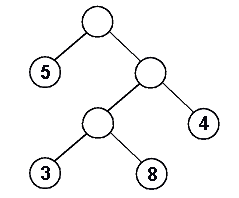
\includegraphics[width=4.406cm,height=3.667cm]{image/a2012Logique2eme-img036.png}  &
			~

			~

			~

			{ devient après remplissage [F0E0?]} &
			 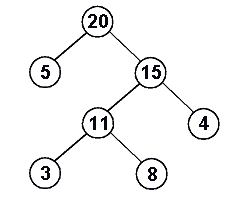
\includegraphics[width=4.773cm,height=3.955cm]{image/a2012Logique2eme-img037.png} \\
			\end{supertabular}
			\end{flushleft}

		\end{Exercice}
		
		\begin{Exercice}{Combien de valeurs~?}
			Écrire un algorithme qui indique le nombre de valeurs différentes 
			que contient un arbre.
		\end{Exercice}
		
	\subsection{Arbres binaires}
	%===========================

		\begin{Exercice}{Arbre binaire équilibré}
			Dans un arbre binaire, on définit le \textbf{facteur d'équilibre} 
			d'un n{\oe}ud de la façon suivante~: c'est la différence entre 
			la hauteur de son sous-arbre gauche et celle de son sous-arbre droit. 
			On dit que l'arbre est \textbf{équilibré} si, pour tout n{\oe}ud 
			de l'arbre, ce facteur d'équilibre est compris entre --1 et 1.
		\end{Exercice}
		
		\begin{Exercice}{Arbre binaire pair}
			Un arbre binaire est \textbf{pair} si chacun de ses n{\oe}uds 
			a soit 2 fils, soit aucun. Écrire un algorithme qui
			vérifie si un arbre binaire possède cette propriété. 
			
			N. B.~: un arbre vide est pair.
		\end{Exercice}
		
		\begin{Exercice}{OXO}
			Soit un arbre binaire de caractères. Vérifier s'il contient 
			la configuration 'O'-'X'-'O' formée respectivement par un
			fils gauche, un père et un fils droit.
		\end{Exercice}

		\begin{Exercice}{Arbre binaire symétrique}
			Écrire un algorithme qui vérifie si un arbre binaire est 
			\textbf{symétrique}, c'est-à-dire si le sous-arbre gauche de la
			racine est identique en miroir à son sous-arbre droit.

			\begin{center}
			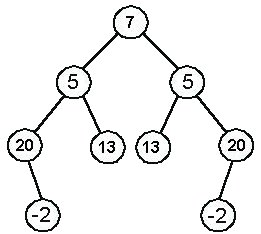
\includegraphics[width=4.805cm,height=4.307cm]{image/a2012Logique2eme-img038.jpg}
			\end{center}
		\end{Exercice}
		
	\subsection{Arbres binaires ordonnés}
	%====================================

		\begin{Exercice}{L'arbre binaire est-il ordonné~?}
			Écrire un algorithme qui vérifie si un arbre binaire est ordonné.
		\end{Exercice}
		
		\begin{Exercice}{Le maximum}
			Écrire un algorithme qui retourne la valeur maximum d'un arbre 
			binaire ordonné.
		\end{Exercice}
		
		\begin{Exercice}{Recherche dichotomique}
			Écrire un algorithme qui recherche dans un arbre binaire la 
			présence d'un n{\oe}ud de valeur donnée, et en retourne
			l'accès. Si la valeur ne se trouve pas dans l'arbre, 
			l'algorithme retourne \textit{rien} dans ce cas.
		\end{Exercice}
		
		\begin{Exercice}{Ajout de valeur}
			Écrire un algorithme qui ajoute un n{\oe}ud dans un arbre 
			binaire ordonné, dont la valeur est entrée en paramètre.
		\end{Exercice}
		
	\subsection{Arbres quelconques}
	%==============================
			
			\begin{Exercice}{Le dictionnaire}
				Utilisons un arbre pour stocker les mots d'un dictionnaire. 
				Les lettres d'un mot sont représentées chacune par
				un n{\oe}ud à un niveau différent et les mots ayant 
				le même début partagent leurs n{\oe}uds. De plus, un caractère
				spécial indique la fin d'un mot. La racine ne contient 
				rien. Les fils d'un n{\oe}ud ne sont pas forcément dans 
				l'ordre	alphabétique.
				
				Dans l'exemple ci-dessous, le dictionnaire contient les mots 
				AI,~AIL, {dots}, AS, SA, {dots}, SOT, Y.
				\begin{center}
				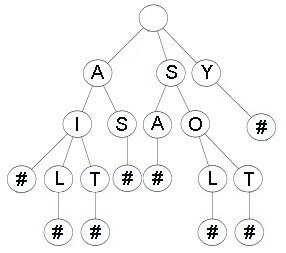
\includegraphics[width=6.999cm,height=6.195cm]{image/a2012Logique2eme-img039.jpg}
				\end{center}
				
				Écrire un algorithme~:
				
				\begin{enumerate}
					\item {
						qui affiche tous les mots du dictionnaire}
					\item {
						qui ajoute un mot dans le dictionnaire}
					\item {
						qui enlève un mot du dictionnaire}
				\end{enumerate}
			\end{Exercice}
			
			\begin{Exercice}{Au fil de l'eau}
				Les cours d'eau d'un bassin fluvial peuvent être schématisés 
				avec un arbre~: la racine contient le nom du fleuve, 
				et les fils d'un n{\oe}ud sont les affluents du fleuve 
				ou des rivières faisant partie du bassin fluvial.
				\begin{center}
				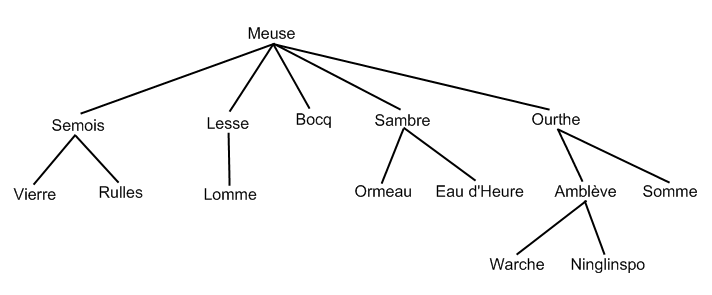
\includegraphics[width=11.529cm,height=4.768cm]{image/a2012Logique2eme-img040.png}
				\end{center}
				Écrire un algorithme qui reçoit le nom d'un cours d'eau 
				en paramètre et affiche la suite des rivières qui
				le conduisent au fleuve principal. Par exemple, 
				pour \textit{«~Somme~»}, l'algorithme affiche \textit{«~Somme~»}, 
				\textit{«~Ourthe~»} et \textit{«~Meuse~»}.
			\end{Exercice}
								